\subsection{Ca sử dụng thêm mục lưu trữ vào chuyến đi}
\noindent Ca sử dụng này mô tả cách người dùng lưu các địa điểm, sự kiện, hoặc nhà hàng vào một chuyến đi cụ thể để tham khảo khi lên lịch trình. Người dùng có thể tìm kiếm và chọn các mục muốn lưu. Bảng~\ref{tab:uc_add_saved_item_spec} trình bày chi tiết đặc tả ca sử dụng, bao gồm luồng sự kiện chính, luồng thay thế, các điều kiện và yêu cầu liên quan. Các biểu đồ hoạt động, quan hệ (Bảng~\ref{tab:uc_add_saved_item_diagrams}) và tuần tự (Hình~\ref{fig:3-3-12-sequence-diagram}) minh họa rõ hơn về quy trình và tương tác hệ thống.
% \vspace{0.5cm} % Adjust spacing if needed

% Use longtable environment
% Need \usepackage{longtable} and \usepackage{calc} in preamble
\begin{longtable}{| p{4cm} | p{\dimexpr\linewidth-4cm-4\tabcolsep} |} % Adjust widths as needed
    \caption{Đặc tả ca sử dụng thêm mục lưu trữ vào chuyến đi} % Caption inside longtable (no period)
    \label{tab:uc_add_saved_item_spec} \\ % Label after caption

    \hline
    \textbf{Mô tả} & Người dùng có thể lưu các địa điểm, sự kiện, nhà hàng vào chuyến đi để lên lịch trình dựa trên nó. \\
    \hline
    \endfirsthead % Header for the first page

    % No \endhead content needed

    % No \endfoot content needed

    \hline % Footer for the last page
    \endlastfoot

    % --- Table Content ---
    \textbf{Luồng cơ bản} & 1. Người dùng chọn một chuyến đi muốn thêm mục lưu. \newline
                           2. Hệ thống lấy dữ liệu chi tiết của chuyến đi và hiển thị. \newline
                           3. Người dùng bấm "Thêm mục lưu". \newline
                           4. Hệ thống điều hướng sang trang thêm mục lưu và hiển thị thanh tìm kiếm. \newline
                           5. Người dùng nhập tên địa điểm, sự kiện hoặc nhà hàng muốn thêm vào chuyến đi. \newline
                           6. Hệ thống tìm kiếm và hiển thị danh sách các mục lưu phù hợp với từ khóa tìm kiếm. \newline
                           7. Người dùng chọn mục muốn lưu trong danh sách. \newline
                           8. Hệ thống thông báo đã thêm thành công. \\
    \hline
    \textbf{Luồng thay thế} & Người dùng bấm vào mục đã lưu sẽ bỏ lưu mục đấy. \\
    \hline
    \textbf{Tiền điều kiện} & - Người dùng đang đăng nhập và phiên đăng nhập chưa kết thúc.\newline
                           - Người dùng đã tạo hoặc tham gia ít nhất một chuyến đi. \newline
                           - Trạng thái chuyến đi khác "Đã hoàn thành" và "Hủy". \\
    \hline
    \textbf{Hậu điều kiện} & - Hệ thống thêm mục lưu của chuyến đi vào cơ sở dữ liệu.\newline
                           - Người dùng có thể xem lại mục lưu đã thêm vào chuyến đi. \\
    \hline
    \textbf{Yêu cầu phi chức năng} & Hệ thống thêm mục lưu dưới 1s. \\
    % --- End Table Content ---

\end{longtable}


\begin{table}[H] % Wrap the diagrams table
    \centering
    \caption{Biểu đồ hoạt động và quan hệ ca sử dụng thêm mục lưu trữ vào chuyến đi} % Add caption (no period)
    \label{tab:uc_add_saved_item_diagrams} % Add label
    \begin{tabular}{| c | c |}
        \hline
        \textbf{Biểu đồ hoạt động} & \textbf{Quan hệ} \\
        \hline
        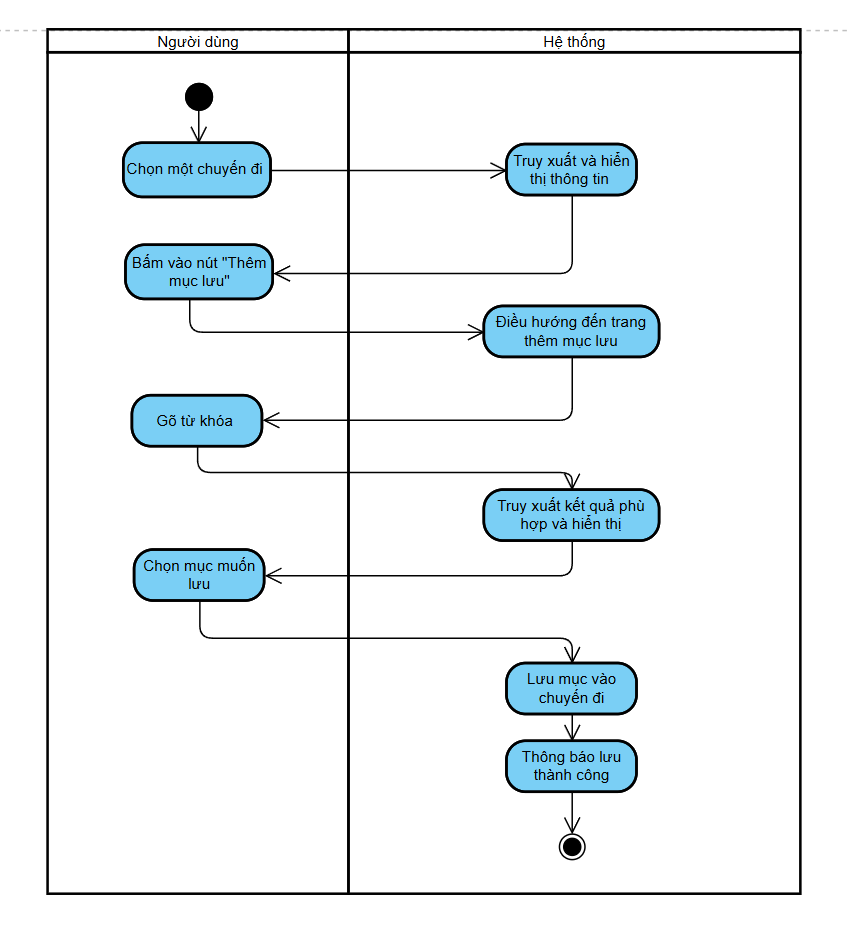
\includegraphics[width=0.5\linewidth]{figures/c3/3-3-12-ad.png} % Specified width
        &
        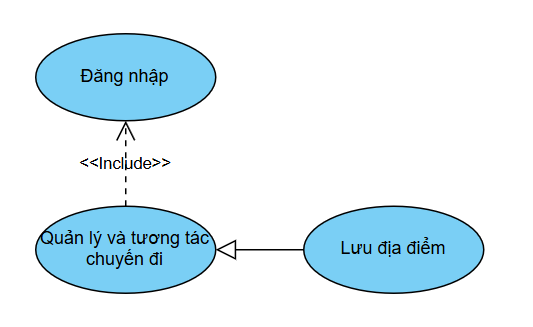
\includegraphics[width=0.45\linewidth]{figures/c3/3-3-12-rd.png} \\ % Specified width
        \hline
    \end{tabular}
\end{table}

\begin{figure}[H]
    \centering
    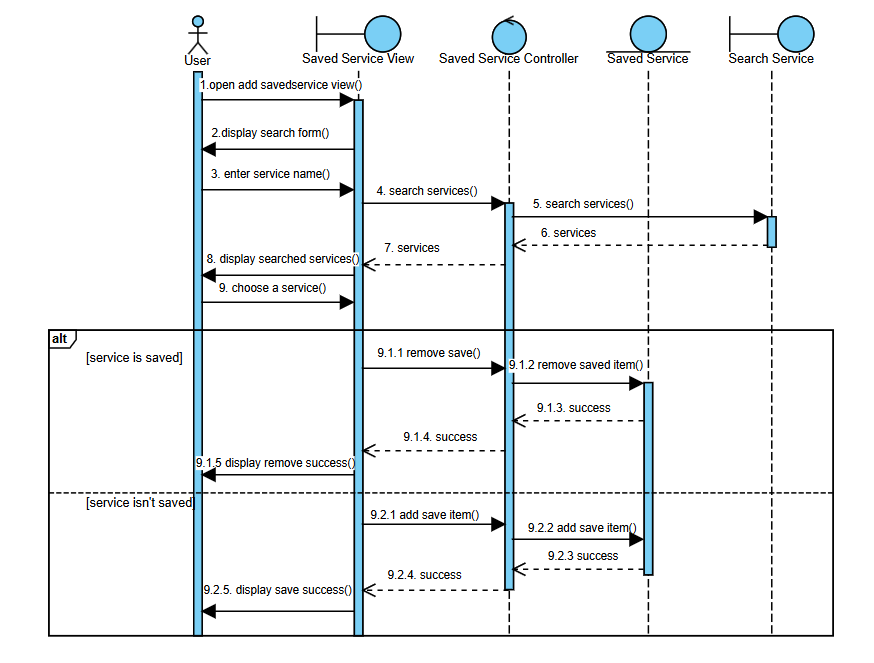
\includegraphics[width=0.92\textwidth]{figures/c3/3-3-12-sd.png} % Specified width
    \caption{Biểu đồ tuần tự ca sử dụng thêm mục lưu vào chuyến đi.} % (no period)
    \label{fig:3-3-12-sequence-diagram}
\end{figure}